\documentclass[architecture]{compas2018}
%%%%%%%%%%%%%%%%%%%%%%%%%%%%%%%%%%%%%%%%%%%%%%%%%%%%%%%%%%%%%%%%%%%%%
\usepackage{url}
\toappear{1} % Conserver cette ligne pour la version finale

\usepackage{tikz}
\usetikzlibrary{arrows.meta}
\tikzset{
  hwblock/.style={draw, rectangle, rounded corners=.3, very thick, fill=black!5, font=\sf, minimum height=5ex},
  hwbus/.style={very thick,>=stealth},
  hwwire/.style={thick,>=stealth},
  hwword/.style={draw, rectangle, minimum height=3ex},
  bitwidth/.style={font=\scriptsize,midway,right}
}

\newcommand{\reg}{\textit{reg}}
\newcommand{\const}{\textit{const}}
\newcommand{\shiftval}{\textit{shiftval}}
\newcommand{\cond}{\textit{cond}}
\newcommand{\ctr}{\textit{ctr}}
\newcommand{\size}{\textit{size}}
\newcommand{\addr}{\textit{addr}}

\newcommand{\todo}[1]{\textcolor{red}{TODO: #1}}
\begin{document}

\title{Une architecture minimisant les échanges\\ entre processeur et mémoire}

\author{Florent de Dinechin, \\Sébastien Michelland, Maxime Darrin, Antonin Dudermel, Alban Reynaud}

\address{
  % \begin{tabular}{cc}
  %   ENS-Lyon & INSA Lyon \\
  %   \texttt{nom.prenom@ens-lyon.org} \\
  % \end{tabular}
}

\date{\today}

\maketitle
\sloppy

\begin{abstract}
  Dans une architecture de von Neumann, les échanges de données représentent le gros de l'énergie dépensée.
Or le processeur communique avec la mémoire au moyen d'un bus d'adresse et d'un bus de données de grandes tailles (entre 8 et 64 bits).
Cette granularité contraint ces échanges, et en particulier l'encodage des instructions du processeur.
Cet article étudie ce qui est possible en levant cette contrainte.
Il propose une architecture 64 bits dont la mémoire est adressable par bit, ce qui permet des instructions de taille arbitraire.
Pour ne pas devoir envoyer une adresse complète à la mémoire à chaque accès, la solution proposée est l'usage de pointeurs auto-incrémentés dupliqués dans la mémoire et le processeur.

Cet article décrit aussi une expérience pédagogique réalisée à l'ENS-Lyon.
Un premier jeu d'instruction a été défini en TD et son encodage choisi à la main.
Ceci a permis aux étudiants d'écrire en binôme un assembleur et un simulateur, puis plusieurs milliers de lignes de programmes allant du petit noyau de calcul au jeu vidéo et à l'émulateur.
Sur les traces de ces programmes, on a pu ensuite calculer un encodage optimal des instructions en fonction de leur fréquence, et les comparer à l'encodage initial.
 Ces expérimentations ont aussi montré les limites de cette première approche, et l'article discute  des solutions pour y remédier.
\end{abstract}

%=========================================================
\section{Introduction et motivation}
% =========================================================
Cet article s'intéresse à l'encodage du jeu d'instruction d'un processeur de von Neumann, interfacé à une mémoire par un bus d'adresse et un bus de données  (figure~\ref{fig:mvn}).

\newcommand{\figVonNeumann}{
  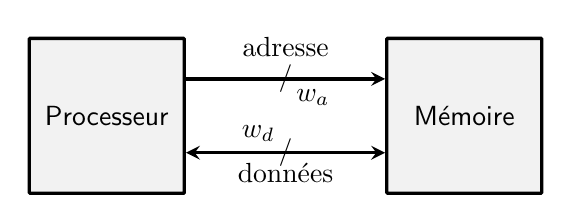
\begin{tikzpicture}
    \node[hwblock, minimum width=13ex,minimum height=13ex] (p) at (0,0)  {Processeur} ;
    \node[hwblock, minimum width=13ex,minimum height=13ex] (m) at (30ex,0)  {Mémoire} ;
    \draw[hwbus,->] (p.25) -- (m.155) node[midway,above=1ex]{adresse} node[midway]{/} node[midway, below right]{$w_a$};
    \draw[hwbus,<->] (p.335) -- (m.205) node[midway,below]{données} node[midway]{/} node[midway, above left]{$w_d$};
  \end{tikzpicture}
}

\begin{figure}[b]
  \begin{center}
    \figVonNeumann
  \end{center}
  \caption{Une machine de von Neumann.}
  \label{fig:mvn} \index{von Neumann}\index{machine de von Neumann}
\end{figure}

Le jeu d'instruction d'un tel processeur (Instruction Set Architecture ou ISA) reflète l'état de la loi de Moore à l'époque de sa conception.
Celle-ci se traduit par exemple par un doublement de la quantité de mémoire intégrée sur une puce tous les deux ans.
Comme il faut bien adresser cette mémoire, le bus mémoire suit, et sa taille ($w_a$ sur la figure) grandit donc d'un bit tous les deux ans.
Ceci se traduit à son tour par une croissance de la taille des registres qui, dans un processeur, peuvent adresser la mémoire.
Toutefois, cette croissance a suivi des puissances de 2: de 8 bits aux temps héroïques à 16 bits dans les années 1970, 32 bits dans les années 1980, et 64 bits dans les années 2000, et sans doute pour encore quelques dizaines d'années.

\iffalse % c'est fort intéressant mais on s'en fout
La croissance du bus de données a suivi avec du retard, pour plusieurs raisons.
La première est que la loi de Moore doit aussi fournir assez de transistors au processeur pour calculer sur des données de plus en plus grandes.
Mais la complexité des principales opérations d'un processeur travaillant sur $n$ bits est en $n$, en $n\log n$ ou au pire en $n^2$: si l'on a pu être à l'étroit jusque dans les années 90 pour construire un processeur qui peut calculer sur des adresses mémoires, ce n'est plus le cas depuis.
La seconde raison est que les ordinateurs servent beaucoup à travailler sur du texte, donc des octets.
On a donc vu des processeurs très populaires 8/16 bits, c'est à dire $w_d=8$ et  $w_a = 16$: les z80, 6502, 8088; des processeurs 16/32 bits (68000, 80286 à 486); et même une variante 8/32 bits, le 68008. Puis l'industrie a convergé vers 32/32 avec l'arrivée des processeurs RISC  (SPARC,  ARM et Power)  puis et 64/64 avec AMD64 et ARM64.
Ainsi,  
De nos jours, les processeurs ont des registres de plusieurs centaines de bits (AMD64 SSE* puis AVX*, ARM Neon), encore une fois parce que la loi de Moore le permet.
Mais ces registres sont des vecteurs de données d'au plus 64 bits.
\fi



Une question intéressante, et qui commence à toucher le jeu d'instruction, est  la granularité à laquelle on peut adresser la mémoire.
L'ancêtre 4004 et le processeur Saturn des calculettes HP adressaient leur mémoire par case de 4 bits: ceci correspondait au besoin du décimal codé en binaire.
La plupart des processeurs (dont les Intel/AMD de nos PC et les ARM de nos gadgets) adressent leur mémoire par octet pour être efficaces sur le traitement de texte.

% \subsection{Pourquoi pas l'adressabilité au bit près?}
Ceci nous amène à la première constatation. Dès lors que les adresses font 64 bits, on peut parfaitement décider  que le adresses seront des adresses de bits.
On perd juste un facteur 8 en quantité de mémoire adressable.
Ce qui aurait été inacceptable à l'époque des adresses sur 16 bits est actuellement indolore: avec un espace d'adressage sur 64 bits, il reste tout de même $2^{61}\approx 2.10^{18}$ bits, ou 2 exabits, à adresser.


Attention, on parle ici de l'abstraction offerte par le jeu d'instruction, pas de l'interface physique.
Les deux sont déjà différentes dans les processeurs actuels.
Si l'ISA définit une mémoire adressable par octet, l'accès physique à la mémoire se fait à travers un cache qui, côté processeur, offre l'adressage par octet, mais côté mémoire physique  réalise des accès alignés sur une grande puissance de 2 correspondant à la taille de la ligne de cache.
%Ceci explique aussi les contraintes d'alignement pour les données de grande taille.
 On peut estimer que passer d'un adressage par octet à un adressage au bit ajoute trois niveaux de multiplexeurs au décodage de la ligne de cache, un changement plus quantitatif que qualitatif.


Ce qu'on gagne à avoir une adresse pour chaque bit, c'est que la taille des données et des instructions peut être variable au bit près: on peut espérer n'envoyer que les bits utiles.
Comme exemple d'application, on peut citer les UNUM, un format de représentation des nombres flottants de taille variable et auto-descriptif (les tailles d'exposant et de mantisse sont encodées dans un en-tête) proposé par  Gustafson en 2015 \cite{2015-02-GUSTAFSON}.
Cette proposition est déjà abandonnée par son auteur \cite{2016-09-TICHY} malgré quelques bonnes idées, mais une de ses  motivations reste: 
d'après Dally, \emph{fetching operands costs more than computing on them}, et l'on parle d'un facteur 1000 \cite{Dally:SC2010}.


Il y a aussi des applications, comme les réseaux de neurones, qui se contentent très bien de données sur de très petites précision, voire des données binaires \cite{AndriCRB16,AlemdarEtAl2017:TernaryCNN,AmiriEtAl2018:mixedPrecCNN,Preusser:DATE2018:heteroCNN}. 

Attention, il ne faut pas que l'on ait à envoyer 64 bits d'adresse pour chaque bit de données échangé, ce qui serait bien pire que le faire pour chaque octet. 
Reprendre la figure \ref{fig:mvn} en fixant juste $w_d=1$ serait contre-productif.

Ce travail essaye d'imaginer une architecture (au sens ISA) dans laquelle on peut tailler instructions et données au bit près, et ne payer que pour les bits effectivement transférés.
Il a été réalisé dans le cadre de l'enseignement de l'architecture en L3 à l'ENS-Lyon: les développements et les expériences présentées sont l'aboutissement de séances de travaux dirigés et de devoirs à la maison\footnote{Le lecteur trouvera les supports correspondant ici: \url{perso.citi-lab.fr/fdedinec/enseignement/2017/ASR1/}}. 

\iffalse
\subsection{Pourquoi pas un jeu d'instruction au bit près?}

Les jeux d'instructions les plus compacts à notre connaissance sont les \emph{bytecodes} des machines virtuelles comme Java ou Python, qui émulent une machine à pile.
\todo{F2D}

\subsection{Contexte de ce travail}
Résumé des objectifs pédagogiques du cours ASR1

\todo{F2D}
\subsection{Plan}

\todo{F2D}
\fi


\section{Architecture générale et interface mémoire}
Pour concrétiser l'adressabilité au bit près, nous proposons une interface processeur-mémoire strictement série représentée sur la figure~\ref{fig:overview}.
Les données passent en série, bit à bit, sur le fil \texttt{D}.
Le processeur contrôle le sens de transfert par les fils \texttt{Read} et \texttt{Write}.
Pour ne pas avoir à transmettre une adresse de $n$ bits par bit de donnée, les adresses sont le plus souvent implicites.
Dans ce but, on a 4 compteurs, répliqués dans le processeur et la mémoire.
Le pointeur de programme, PC, est l'un de ces compteurs.
Il s'auto-incrémente, classiquement, au cours de la lecture d'une instruction et pour passer à l'instruction suivante.

Pour lire une donnée, le processeur sélectionne un des compteurs en positionnant les deux bits  \texttt{Select}.
Puis il lève \texttt{Read}.
Tant que \texttt{Read} vaut 1, le compteur sélectionné s'incrémente (côté processeur comme côté mémoire) et les bits qu'il pointe sont transférés sur le fil \texttt{D}.
Lorsque le processeur décide qu'il a lu toute une donnée, il baisse \texttt{Read}.
Le mécanisme est similaire en cas d'écriture.

Les instructions de lecture/écriture mémoire ne donnent pas d'adresse, mais précisent un compteur (encodé sur 2 bits) et le nombre de bits mémoire à lire/écrire (parmi 1, 4, 8, 16, 32 et 64 bits, encodé par un code prefix-free sur 2 ou 3 bits).
Il faut aussi des instructions qui permettent de transférer un registre dans un compteur ou inversement.
Ces instructions ont un encodage compact (le code op, suivi du registre encodé sur 3 bits et du compteur encodé sur 2).
Par contre, leur exécution provoque bien plus de transferts de bits: par exemple pour changer un compteur, le processeur lève \texttt{SetCounter}, puis transfère sur \texttt{D} les bits du compteur sélectionné par \texttt{Select}, poids faibles en tête.
Lorsque le processeur baisse \texttt{SetCounter}, la mémoire complète le compteur avec le dernier bit transmis (extension de signe).
Si le compteur était le PC, on a réalisé un saut.

Cette interface ne dépend pas de la taille mémoire, ni de la puissance du processeur (elle est identique pour un processeur 32 ou 64 bits).
\begin{figure}[h]
    \begin{center}
  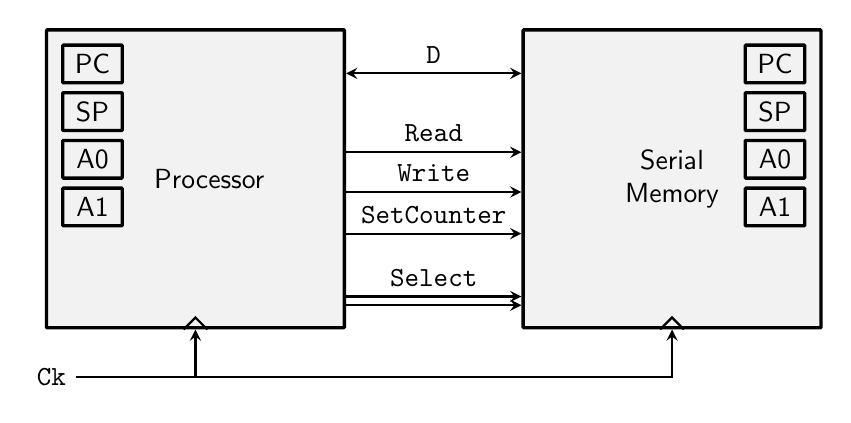
\begin{tikzpicture}
    \node[hwblock, minimum width=25ex,minimum height=25ex] (p) at (-10ex,0)  {~~~Processor} ;
%    \draw  (p) ++(0,-10ex)  node {} ;
    \node[hwblock, minimum width=25ex,minimum height=25ex, align=center] (m) at (30ex,0)  {Serial\\ Memory} ;
    
    \draw (p.north west)  ++(4ex,-3ex)  node[hwblock,minimum height=3ex,minimum width=5ex]{PC} ;
    \draw (p.north west)  ++(4ex,-7ex)  node[hwblock,minimum height=3ex,minimum width=5ex]{SP} ;
    \draw (p.north west)  ++(4ex,-11ex)  node[hwblock,minimum height=3ex,minimum width=5ex]{A0} ;
    \draw (p.north west)  ++(4ex,-15ex)  node[hwblock,minimum height=3ex,minimum width=5ex]{A1} ;
    
    \draw (m.north east)  ++(-4ex,-3ex)  node[hwblock,minimum height=3ex,minimum width=5ex]{PC} ;
    \draw (m.north east)  ++(-4ex,-7ex)  node[hwblock,minimum height=3ex,minimum width=5ex]{SP} ;
    \draw (m.north east)  ++(-4ex,-11ex)  node[hwblock,minimum height=3ex,minimum width=5ex]{A0} ;
    \draw (m.north east)  ++(-4ex,-15ex)  node[hwblock,minimum height=3ex,minimum width=5ex]{A1} ;

    \draw[hwwire,<->] (p.35) -- (m.145) node[midway,above]{\texttt{D}};

    \draw[hwwire,->] (p.10) -- (m.170) node[midway,above]{\texttt{Read}};
    \draw[hwwire,->] (p.355) -- (m.185) node[midway,above]{\texttt{Write}};
    \draw[hwwire,->] (p.340) -- (m.200) node[midway,above]{\texttt{SetCounter}};
    \draw[hwwire,->] (p.322) -- (m.218) node[midway,above]{\texttt{Select}};
    \draw[hwwire,->] (p.320) -- (m.220) node[midway,above]{};
    \draw[hwwire,<-] (m.south) -- ++(0,-4ex) -- ++(-50ex,0) node[left]{\texttt{Ck}};
    \draw[hwwire,<-] (p.south) -- ++(0,-4ex);
    \draw[hwwire,-] (p.south)  ++(-1ex, 0) -- ++(1ex,1ex) -- ++(1ex,-1ex); % horloge
    \draw[hwwire,-] (m.south)  ++(-1ex, 0) -- ++(1ex,1ex) -- ++(1ex,-1ex); % horloge
  \end{tikzpicture}
  \end{center}
  \caption{L'interface processeur-mémoire proposée}
  \label{fig:overview}
\end{figure}

\subsection{Comparaison avec une architecture classique}
Si l'on compare la figure~\ref{fig:overview} avec la figure~\ref{fig:mvn} lors de l'exécution d'un programme classique, il est clair que notre proposition dégrade le temps d'exécution, puisque la transmission de la moindre instruction et de la moindre donnée demande plusieurs cycles d'horloge.

Si par contre on s'intéresse au nombre de transitions sur les fils (une métrique raisonnable pour mesurer la consommation dynamique), on peut faire les observations suivantes.

\begin{itemize}
\item Dans la lecture de données consécutives en mémoire, notre proposition fait l'économie de toutes les transitions sur le bus d'adresse.
  En particulier, la lecture des instructions d'un programme, hors branchements,  ne demande aucune transmission d'adresse.
\item Adresses comme données peuvent être transmises au bit près.
\item Par contre on a une transition d'horloge par bit transmis, au lieu d'une transition d'horloge pour $w_a$ ou $w_d$ bits.
\end{itemize}
Il y a donc un potentiel de réaliser moins de transitions avec le système proposé, potentiel que le présent article se propose de mesurer.

Pour cela nous nous efforçons principalement de minimiser la taille de l'encodage du jeu d'instructions.

\subsection{un c\oe ur  RISC}
Pour le reste, le processeur embarque un c\oe ur RISC très classique, d'architecture load/store, à 8 registres 32 ou 64 bits.  
Le choix de 8 registres seulement est arbitraire et discutable: il est motivé par des raisons pédagogiques (faire en sorte que les étudiants soient à l'étroit dans les registres  dès l'écriture de programmes simples) et par une raison pratique: encoder le numéro de registre sur aussi peu de bits que possible.
Il est rediscuté en \ref{sec:amelioration}. 


\section{Présentation du jeu d'instruction initial}
Le jeu d'instruction décrit dans cette section est l'aboutissement des deux séances de TD dans lesquelles on a essayé de discuter les tenants et les aboutissants de chaque décision.
Les choix faits ne sont pas toujours ceux qui étaient considérés comme les meilleurs: nous avons aussi privilégié la faisabilité dans le temps limité consacré au module d'ASR1.
% \subsection{Généralités sur les jeux d'instructions}
% Les jeux d'instructions les plus compacts à notre connaissance sont les \emph{bytecodes} des machines virtuelles comme Java ou Python, qui émulent une machine à pile.
% \todo{blabla}

\subsection{Format général des instructions}
Les instructions commencent toutes par un code opération (opcode), suivi des éventuels opérandes.
Les mnémoniques sont écrits exactement dans le même ordre (voir la figure~\ref{fig:exempleasm} pour un exemple).  
Une fois que le processeur a reçu l'opcode, il sait combien d'opérande il doit recevoir et quel est leur type.


Les instructions ALU viennent en version 2 et 3 opérandes, la destination venant toujours en premier.
Par exemple, \\
  \begin{tabular}{lcl}
 \texttt{add2 r0 r1}&& réalise $r_0 \leftarrow r_0+r_1$. \\
 \texttt{add3 r0 r1 r2}&& réalise $r_0 \leftarrow r_1+r_2$.
  \end{tabular}
  
  Dans les programmes écrits à la main, il faut constater qu'on a utilisé surtout les versions à 2 opérandes.
  Ceci est similaire à l'évolution du jeu d'instruction ARM vers le mode Thumb2 qui permet d'encoder sur 16 bits des instructions à deux opérandes. 
  
 L'opcode est différent pour les opérations dont les deux opérandes  sont des registres (par exemple \texttt{add2}), et les opérations portant sur un registre et une constante (par exemple \texttt{add2i}).

Il y a des opcodes de différentes tailles (mais sans préfixe commun, le décodage n'est jamais ambigu)  et les opérandes peuvent également être de différentes tailles.
En particulier, les constantes commencent par un préfixe qui décrit le nombre de bits sur lequel est encodé la constante: voir la table~\ref{tab:constantes} en annexe.
Ainsi les petites constantes courantes comme 0 et 1 sont encodées sur peu de bits, alors que les grandes constantes son également encodables.
Pour les sauts relatifs, on paiera moins cher les sauts proches (jusqu'à +/- 128 bits, soit une dizaine d'instructions) que les sauts plus distants, qui sont par définition pris moins fréquemment.

On a un encodage des constantes différent pour chaque classe d'instruction (table~\ref{tab:constantes}), puisque les besoins ne sont pas les même.


\begin{table}
  \label{tab:constantes}
  \centering
  \caption{Encodage \emph{prefix-free} des différentes constantes}
  \begin{tabular}{|l||l||l|}
    \hline
    adresses et déplacements & constantes ALU & constantes de shift                   \\
    \hline
    0 + 8 bits              & 0 + 1 bit      & 0 + 6 bits  (constante entre 0 et 63) \\
    \hline         
    10 + 16 bits            & 10 + 8 bits    & 1  (constante 1)                      \\
    \hline                  
    110 + 32 bits           & 110 + 32 bits  &                                       \\
    \hline                  
    111 + 64 bits           & 111 + 64 bits  &                                       \\
    \hline
  \end{tabular}
\end{table}

\begin{figure}
  \centering {\small \tt
  \begin{tabular}{llll}
    \textrm{étiquette} & \textrm{mnémonique} & \textrm{encodage initial} & \textrm{encodage Huffman} \\
    \hline
    
         & leti	r0 17        & 0111 000 1000010001 & 100 000 1000010001 \\
         & leti	r1 42        & 0111 001 1000101010 & 100 001 1000101010 \\
         &                   &                     &                    \\
				 & leti	r2 0				 & 0111 010 00				 & 100 010 00       	\\
nonzero: & shift	right r0 1 & 1000 1 000 1				 & 00 1 000 1       	\\
				 & jumpif	nc next		 & 1011 101 000001010	 & 01 101 000001010 	\\
				 & add2	r2 r1				 & 0000 010 001				 & 1010 010 001     	\\
next:		 & shift	left r1 1	 & 1000 0 001 1				 & 00 0 001 1       	\\
				 & cmpi	r0 0				 & 0101 000 00				 & 11 000 00        	\\
				 & jumpif	nz nonzero & 1011 001 010111011	 & 01 001 011000101 	\\
         &                   &                                          \\
loop:    & jump	loop         & 1010 011110011      & 10110 011110010    \\
  \end{tabular}
}
  \caption{Un exemple de programme assembleur (une multiplication entière)}
  \label{fig:exempleasm}
\iffalse
  let r0 17        ; 0111 000 1000010001 ; 000 encode r0,  17 est encodé sur 10 bits
boucle:	                                 ; ceci est une étiquette (label)
  sub2i r0 1       ; 0011 000 01         ; 000 encode r0, 01 encode la constante 1
  jumpif nz boucle ; 1011 001 011100111  ;jumpif nz -25, encodé en 16 bits en tout 
\fi
\end{figure}


%
\iffalse
Les instructions de branchement sont relativement classiques.
\subsection{Les instructions de branchement }
\label{sec:jumpcallret}

Soit $a$ l'adresse du premier bit suivant l'instruction \texttt{jump} ou \texttt{call} (i.e. la valeur du PC lorsqu'il a fini de lire l'instruction et ses opérandes).
Soit $d$ la valeur de déplacement (encodée dans une constante de type \textit{addr}, et signée).

L'instruction \texttt{jump} réalise $\mathtt{pc}\leftarrow a + c$.
L'instruction \texttt{jumpif} aussi, mais seulement si la condition est vraie.

La condition  est encodée sur trois bits  selon la table~\ref{tab:conditions} (ARM utilise 4 bits).

L'instruction \texttt{call} copie $\texttt{a}$ dans $r_{7}$, puis réalise $\mathtt{pc} \leftarrow \texttt{d}$
(\emph{addr} est toujours signé).

L'instruction \texttt{return} copie \texttt{r7} dans \texttt{pc}.


\subsection{Les instructions d'accès mémoire}
\label{sec:mem}



On a 4 compteurs d'adresses, chacun  répliqué dans le processeur et dans la mémoire (Table~\ref{tab:counters}).


Les instructions \texttt{readze}, \texttt{readse} et \texttt{write} lisent ou écrivent le nombre spécifié de bits tout en incrémentant les compteurs correspondant.

On peut émuler une instruction de lecture/écriture mémoire d'un processeur classique en deux instructions: un \texttt{setctr} puis un \texttt{readze} ou \texttt{readse} ou \texttt{write}.

Les instructions \texttt{push} et \texttt{pop} implémentent une pile descendante en mémoire: 
\begin{itemize}
\item \texttt{push} \emph{size} \emph{reg} réalise: \\
   \texttt{setctr} \textit{sp} (\textit{sp} - \textit{size})\\ \texttt{write}  \textit{sp} \textit{size} \textit{reg} \\ \texttt{setctr} \textit{sp} (\textit{sp} - \textit{size})
\item \texttt{pop} \emph{size} \emph{reg} est un raccourci offert par l'assembleur pour \\\texttt{readze} \textit{sp} \emph{size} \emph{reg}\\
  
\end{itemize}

\fi

\section{Premières expériences}
Ces expériences portent sur une petite suite de benchmarks, écrits en assembleur à la main puisque nous n'avons pas encore de compilateur pour cette architecture.
Quelques résultats sont rapportés dans la table~\ref{tab:bitcounts}.

\textbf{Multiplication entière} Le choix d'une ISA sans instruction de multiplication ni division est essentiellement pédagogique, pour faire manipuler l'arithmétique de bas niveau.
les étudiants ont donc dû écrire le programme de la figure~\ref{fig:exempleasm}, et même l'assembler à la main dans un premier temps.
Il n'y a pas d'accès mémoire dans ce benchmark, hors du programme lui-même.
Le c\oe ur de boucle est encodé en 69 bits.
% Pour comparaison, un programme similaire compilé pour le processeur RISC 16 bits MSP430, 10 instructions aussi, consomme  24 octets, soit 192 bits, dont 96 pour le c\oe ur de boucle.
% A l'exécution, 
% Notre encodage est donc clairement plus compact, pour un processeur 64 bits.
% voir le répertoire MSP430




\textbf{Produit de matrice}
C'est un produit de matrices 32x32 d'entiers 64 bits aléatoires.
Ce programme utilise la multiplication entière précédente, mais les matrices sont lues et écrites en mémoire.
On présente deux simulations: la première avec des matrices pleines, et la seconde avec des matrice creuse (en moyenne 90\% de 0).
Les multiplications par 0 terminant instantanément, mais étant tout de même stocké en mémoire comme 64 bits, cette seconde version provoque un rapport bits de données / bits de code plus élevé.

\textbf{Chip8}
Un binôme a écrit un émulateur CHIP8 \cite{Chip8:1978} pour notre système.
Ce benchmark fait tourner le jeu BRIX pendant exactement une minute par partie.
Ce benchmark est très orienté mémoire puisqu'il interagit beaucoup avec l'écran.
Pourtant on voit que les transferts de code restent majoritaires.


La première expérience consiste à utiliser l'encodage initial.
Des compteurs, dans le simulateur, mesurent l'utilisation de chaque instruction.%. (rapportée dans la table~\ref{tab:opcounts}. \todo{Il faut choisir quelle instruction on rapporte}
D'autres compteurs comptent les bits échangés sur les fils à l'exécution.
Les résultats correspondants sont donnés dans la première  ligne pour chaque benchmark dans la table~\ref{tab:bitcounts}.

La seconde expérience (dont les résultats sont donnés sur la seconde ligne pour chaque benchmark dans la table~\ref{tab:bitcounts}) consiste à changer l'encodage initial des opcodes pour un encodage de Hufman optimal \emph{pour ce benchmark}.
%Cet encodage utilise les statistiques de la table~\ref{tab:opcounts}.
L'intérêt de cette seconde expérience est de donner une borne inférieure: l'idée de changer l'encodage des instructions en fonction du programme va au dela de la présente étude.
Du reste, on voit que l'encodage des opcodes peut être amélioré, mais que les gains à espérer restent faibles.


\iffalse
./asm.py -v -b prog/mult.s
./emu/emu -s -t prog/mult.bin
./emu/emu -i prog/mult.bin | ./huffmann.py > mult.huff
./asm.py --loadhuffman mult.huff -v -b prog/mult.s -o  prog/mult.huff.bin
./emu/emu -s -t -lh mult.huff -i prog/mult.huff.bin

python3 ./matmulstat/makematrix.py
./asm.py -v -b prog/matmul.s
./emu/emu -s -t prog/matmul.bin --load 65536:mat32x32.bytes
./emu/emu -i prog/matmul.bin --load 65536:mat32x32.bytes | ./huffmann.py > matmul.huff
./asm.py --loadhuffman matmul.huff -v -b prog/matmul.s -o prog/matmul.huff.bin
./emu/emu -s -t -lh matmul.huff prog/matmul.huff.bin --load 65536:mat32x32.bytes

idem mais avec python3 ./matmulstat/makematrix.py 0.1 pour une matrice creuse

\fi


\begin{table}
  \centering
  \begin{tabular}{|r||c|c|c||c|c|c|c|c||c|}
    \hline
    & \multicolumn{3}{c||}{taille du programme} & \multicolumn{6}{c|}{bits échangés à l'exécution}                    \\
    \hline

    
    benchmark      & instr     & bits       & bpi         & prog    & data R  & data W  & counters & branch  & total      \\
    \hline
    \hline
    binmult~~~I    & 10        & 125        & 12.5        & 89.4\%  &         &         &          & 10,6\%  & 415        \\
     H             &           & 113        & 11.3        & 85.5 \% &         &         &          & 14.5 \% & 373        \\
    \emph{ msp430} & \emph{10} & \emph{192} & \emph{19.2} & --      & --      & --      & --       & --      & \emph{960} \\
    \hline
    \hline
    matmul~~~I     & 112       & 1632       & 14.6        & 80.4 \% & 5.0 \%  & 2.6 \%  & 0.3 \%   & 11.8 \% & 1.72e8     \\ 
     (dense)~  H           & 112       & 1817       & 16.2        & 75.4 \% & 5.6 \%  & 2.9 \%  & 0.3 \%   & 15.9 \% & 154e8      \\ 
    \hline
    matmul~~~I    & 112       & 1632       & 14.6        & 55.3 \% & 23.3 \% & 12.1 \% & 1.2 \%   & 8.0 \%  & 3.68e7     \\ 

    (sparse)~ H & 112 & 1613 & 14.4  & 52.1 \% & 25.2 \% & 13.1 \% & 1.3 \% & 8.3 \% & 341e7\\ 

    \hline
    \hline
    Chip8~~~I     & 768 & 14155 & 18.4 &  64.3 \% & 10.4 \% & 9.7 \% & 7.5 \% & 8.1 \% & 1.068e8       \\
     H    & 768 & 13699 & 17.8 & 63.1 \% & 10.7 \% & 9.9 \% & 7.7 \% & 8.6 \% & 1.063e8\\ 
    \hline
  \end{tabular}
  \caption{Nombre de bits échangés par benchmark. Encodage des opcodes: I initial, H Huffman. Les colonne à partir de \emph{data R} comptent  les bits qui passent sur \texttt{D} à l'exécution des instructions de lecture, d'écriture, d'accès aux compteurs, et de sauts/call  respectivement. }
  \label{tab:bitcounts}
\end{table}


%Nous concluons en definissant quelques pistes d'amélioration.


\iffalse
\subsection{Modes d'adressage mémoire}
\subsubsection{Choix initiaux}
On a fait le choix de ne pas faire d'adressage par registre : en effet, cela aurait coûté 64 bits d'adresse par adressage. Les compteurs permettent de faire autant avec seulement 2 bits à chaque adresse. En contrepartie, l'arithmétique sur les pointeurs devient extrêmement coûteuse : charger une adresse dans un registre ; faire une opération arithmétique ; affecter l'adresse avec le registre. Cependant, on espère que la plupart du temps, les données sont lues de manière séquencielle, et que donc un adressage avec post-incrément suffit à limiter l'arithmétique des pointeurs. Cette affirmation est relativisée en \ref{addr:amel}  
\subsubsection{Améliorations\label{addr:amel}}
Même avec le dédoublement des compteurs dans le processeur, la plupart des opérations restent coûteuses, surtout le \texttt{push}, qui nécessite de déplacer deux fois un compteur à cause du post-incrément. Une première idée est d'ajouter la possibilité d'écrire en mémoire avec pré-décrément (on a assez de fils pour indiquer à la mémoire un sens de lecture). Ainsi, le \texttt{push} ne nécessite plus de déplacer de pointeurs.\par
Un autre problème est l'envoi systématique de $64$ bits pour synchroniser les compteurs. En effet, si un compteur est à \texttt{0x10040}, pour le déplacer à \texttt{0x10000}, il suffit de mettre les 7 premiers bits à 0. On a ainsi un gain énorme (ici 57 bits) sur les petits sauts. La table \ref{tab:costs} résume les gains obtenus pour les différentes améliorations.


\section{Améliorations et pistes d'améliorations \label{sec:amelioration}}
\subsection{Combien de registres ?}
Le nombre de registres est un compromis entre le nombre d'accès à la pile en mémoire et la taille des instructions :
d'un côté, doubler le nombre de registres demande d'ajouter un sinon deux bits à presque toutes les instructions;
de l'autre, avoir trop peu de registres oblige à utiliser plus fréquemment la mémoire.
En survolant les processeurs existant, on peut {\it a priori} considérer que $4$ registres rend le processeur impraticable, et que $16$ est sufisamment confortable pour programmer.
Le choix de 8 est en partie pédagogique: il s'agissait de pouvoir écrire nos premiers programmes assembleur avec assez de registres pour être confortable, et toutefois d'être contraint dès que les programmes deviennent un peu plus gros. 
Avec huit registres, et pas mal d'astuce (par exemple, comment échanger deux registres sans utiliser de registre intermédiaire ?), les élèves s'en sont sortis avec des statistiques de \emph{spill} mémoire raisonnables (inférieures à 1\% des instructions).
Toutefois, une vraie réponse à cette question demande de faire une étude qui couvre également (et surtout) la problématique de la compilation.

Les architectures modernes offrent typiquement entre 16 et 64 registres.
Elles offrent également des mécanismes qui exposent dans le jeu d'instruction un sous-ensemble des registres architecturaux, soit de manière explicite (les fenêtres de registres du SPARC), soit de manière implicite (le techniques de renommage qui permettent l'exécution superscalaire).

On pourrait aussi avoir un nombre de registres beaucoup plus grand avec un encodage compact des registres les plus utilisés.
\todo{relire tout cela}

\subsection{Enrichir l'ISA ?}

L'ISA présentée ici est assez limitée. Elle nous pousse donc à diviser une opération en plusieurs instructions, ce qui rallonge le code et donc le nombre de bits d'instructions échangés. Voici quelques propositions d'améliorations.\par
La principale arithmétique des compteurs est un incrément. Ainsi, en rajoutant des instructions d'incrément de compteurs, on pourrait factoriser \texttt{getctr ctr ri; add2 ri rj; setctr ctr ri} en \texttt{incrctr ctr ri}, gagnant en taille de code, mais aussi l'usage d'un registre. Pour compiler C, on aura aussi besoin d'un accès à la pile indexé par une constante. Enfin, dans une boucle, les \texttt{jump(if)} effectuent des sauts toujours au même endroit. Il serait peut-être intéressant d'avoir des registres \og{} de saut \ \fg{} permettant de stocker l'adresse de saut une fois plutôt que de lire systématiquement une constante à chaque tour de boucle.  
\fi
\section{Conclusion et perspectives d'améliorations}

Les premiers résultats de cette étude sont encourageants, puisqu'on arrive à des encodages d'instructions en moins de 16 bits de moyenne, opérandes compris.
Nous proposons donc une ISA 64 bits dont la taille de code est compétitive avec celle de la génération 8 bits ou des microcontroleurs récents 16 bits.
Nous disposons d'un assembleur et d'un simulateur dans lesquels l'encodage des opcodes est paramétrable, ce qui permet aussi d'ajouter facilement des instructions.



Cette approche s'accomode fort bien d'instructions très disparates en termes d'opérandes.
Ainsi, ajouter une instruction de multiplication-accumulation à 4 arguments ne nous posera pas de problème particulier -- étendre notre ISA avec de telles instructions fait partie des pistes à explorer prochainement.
Ceci fera grossir nos opcodes: pour un jeu d'instruction vraiment complet, nous arriverons peut-être à la conclusion que le \emph{bytecode}, l'adressabilité à l'octet, est un meilleur compromis... c'est celui de l'ISA dominante, où l'instruction \texttt{ret} s'encode toujours en 8 bits, mais plus pour des raisons historiques qu'à la suite d'une savante étude.

Nous nous somme concentrés sur l'encodage des instructions.
Du reste, dans nos expériences, le code représente toujours l'essentiel des bits échangés.
Nous espérons que ce ne sera plus vrai pour un produit de matrices de données 64 bits.

Actuellement, l'arithmétique sur les pointeurs est extrêmement coûteuse, tant en bits d'instructions qu'en bits à l'exécution.
Nous avons commencé à étudier la possibilité de lectures/écritures avec prédécrément pour faciliter le \texttt{push} -- le \texttt{pop}, dans une pile descendante en mémoire, s'accomode très bien de nos pointeurs autoincrémentés.
Il faut aussi étudier un mécanisme simple  d'accès indexé à la pile (SP+constante) pour permettre la compilation efficace de langages de haut niveau (enregistrements d'activation des procédures).
Dans ce cas, on a envie de déléguer à la mémoire l'addition de SP et de la constante pour ne pas les faire transiter sur D dans les deux sens.
Il en va de même pour un saut relatif (addition sur PC d'une constante qui est présente en mémoire dans le code).
Le  \texttt{call addr} est encore pire, puisqu'actuellement, \texttt{addr} passe sur \texttt{D} dans un sens (comme instruction) puis dans l'autre (pour être écrit dans le PC).


La question se pose aussi de la pertinence de ce travail pour construire un ``vrai'' processeur.
Nous sommes conscients que notre  lien série maître/esclave entre processeur et mémoire n'est plus pertinent depuis plusieurs dizaines d'années.
De ce point de vue, ce travail reste théorique.
Cela dit il serait possible d'abriter notre ISA derrière un cache classique, en espérant que la compacité du jeu d'instruction permet d'économiser sur celui-ci.
Il faudrait pour cela montrer que cette économie n'est pas anéantie par le surcoût du décodage de nos encodages \emph{prefix-free}. 


\bibliography{biblio.bib}


\begin{table}[!h]
  \caption{Coûts des opérations}
  \label{tab:costs}
  On propose une première version naïve du coût de chaque opération, pour une architecture 64 bits.
  On distinguera trois types de bits échangées :
  \begin{enumerate}
  \item les instructions du programme (code lu par le processeur).
  \item les données explicitement lues ou écrites (à l'aide de \texttt{readze}, par exemple)
  \item Les bits d'adresses (typiquement, l'affectation de compteurs)
  \end{enumerate}
La taille de l'opcode d'une instruction étant variable, il faut à chaque fois l'ajouter dans les instructions lues.
  \begin{center}
  \begin{tabular}{|l|c|c|c|}
    \hline  
    type & bits d'instruction & bits de données & bits de compteurs \\
    \hline  
    \hline
    \texttt{arith} \reg\ \reg\ & $6$                &    &      \\
    \hline
    \texttt{arith} \reg\ \reg\ \reg\   & $9$   &    &      \\
    \hline
    \texttt{arith} \reg\ \const\       & $3$ + \const       &    &      \\
    \hline
    \texttt{arith} \reg\ \reg\ \const\ & $6$ + \const       &    &      \\
    \hline
    \texttt{r/w} \ctr\ \size\ \reg     & $2$ + \size\ + $3$ & \size           &      \\
    \hline
    \texttt{get-,setctr} \ctr\ \reg\   & $2$ + $3$          &    & $64$              \\
    \hline
    \texttt{jump}         & \addr\             &    & $64$              \\
    \hline
    \texttt{jumpif} \cond & $3$ + \addr\       &    & $0$ ou $64$       \\
    \hline
    \texttt{call} \addr   & \addr\             &    & $64$              \\
    \hline
    \texttt{return}       &       &    & $64$              \\
    \hline
    \texttt{push} \size\ \reg          & $3$   & \size           & $192$             \\
    \hline
  \end{tabular}
  \end{center}
Tableau d'amélioration du nombre de bits de compteurs.
  \begin{center}
    \begin{tabular}{|l|c|c|c|c|}
      \hline  
      type   & sans dédoublement  & initial         & pré-décrément & syncr futée    \\
      \hline  
      \hline
      \texttt{getctr}     & 64  & 0   &   &   \\
      \hline
      \texttt{setctr}     & 64  &     &   & $\leqslant 64$ \\
      \hline
      \texttt{jump(if)}   & 64  &     &   & $\leqslant 64$ \\
      \hline
      \texttt{call}       & 128 & 64  &   & $\leqslant 64$ \\
      \hline
      \texttt{return}     & 64  &     &   & $\leqslant64$  \\
      \hline
      \texttt{push}       & 196 & 128 & 0 &  \\
      \hline
    \end{tabular}
  \end{center}
  Résultat des améliorations sur les benchmarks
  \begin{center}
    \begin{tabular}{|l|c|c|c|c|}
      
      \hline  
      benchmark   & sans dédoubl.  & avec dédoubl.  & pré-décrément & syncro. futée    \\
      \hline  
      \hline
      binmult & 512 & 512 & 512 & 44 \\
      \hline
      matmul & 212018368 & 97.93\% & 95.85\% & 9.75\% \\
      \hline
      matmul* & 35318976 & 87.55\% & 75.09\% & 8.93\% \\
      \hline
      chip8 & 118451648 & 81.98\% & 73.34\% & 14.29\% \\
      
      \hline
    \end{tabular}
  \end{center}

\end{table}

\iffalse

Benchmark pour échanges
(pour binmult matmul)
make
for i in `seq 1 4`
do
./emu/emu --basic prog/binmult.bin -cm $i
done | ./matmulstats/percents.py

for i in `seq 1 4`
do
./emu/emu --basic prog/matmul.bin -cm $i --load 65536:mat32x32.bytes
done | ./matmulstats/percents.py

python3 ./matmulstats/makematrix.py 0.1
for i in `seq 1 4`
do
./emu/emu --basic prog/matmul.bin -cm $i --load 65536:mat32x32.bytes
done | ./matmulstats/percents.py

Chip8 c'est du chrono
$
\fi

\appendix
\begin{table}[!h]
  \caption{Liste des instructions.}
  \label{tab:opcodes}
  Le choix des opcodes est arbitraire.
  Les opérandes d'une instruction suivent l'opcode:
  \begin{itemize}
\item \textit{reg} $\in \{\mathtt{r0}, \mathtt{r1}, ..., \mathtt{r7}\}$ et est encodé par le numéro du registre en binaire.
\item \textit{const}, \textit{shiftval} et \textit{addr} sont définis par la table \ref{tab:constantes}. La colonne \emph{ext} de la table  \ref{tab:opcodes} précise si une constante est étendue avec son signe (s) ou des zéros (z).   
\item  \textit{cond} est une condition portant sur les drapeaux et encodée sur 3 bits.
\item \ctr\ est un des 4 compteurs de la figure \ref{fig:overview}, encodé sur 2 bits.
\item \textit{dir} peut être \texttt{left}, encodé par 0, ou \texttt{right}, encodé par 1.
\end{itemize}
\begin{center}
  \begin{tabular}{|l|l|l|l|l|c|}
    \hline  
    opcode  & mnemonic        & operands                      & description                                          & ext. & {MàJ flags} \\
    \hline  
    \hline  
    0000    & \texttt{add2}   & \reg\ \reg\                   & addition                                             &      & zcvn        \\
    \hline
    0001    & \texttt{add2i}  & \reg\ \const\                 & add immediate constant                               & z    & zcvn        \\
    \hline
    0010    & \texttt{sub2}   & \reg\ \reg\                   & subtraction                                          &      & zcvn        \\
    \hline
    0011    & \texttt{sub2i}  & \reg\ \const\                 & subtract immediate constant                          & z    & zcvn        \\
    \hline
    0100    & \texttt{cmp}    & \reg\ \reg\                   & comparison                                           &      & zcvn        \\
    \hline
    0101    & \texttt{cmpi}   & \reg\ \const\                 & comparison with immediate constant                   & s    & zcvn        \\
    \hline
    0110    & \texttt{let}    & \reg\ \reg\                   & register copy                                        &      &             \\
    \hline
    0111    & \texttt{leti}   & \reg\ \const\                 & fill register with constant                          & s    &             \\
    \hline
    1000    & \texttt{shift}  & \textit{dir} \reg\ \shiftval\ & logical shift                                        &      & zcn         \\
    \hline
    10010   & \texttt{readze} & \ctr\ \size\ \reg\            & read \size\ memory bits (zero-extended) to \reg\     &      &             \\
    10011   & \texttt{readse} & \ctr\ \size\ \reg\            & read \size\ memory bits (sign-extended) to \reg\     &      &             \\
    \hline
    1010    & \texttt{jump}   & \addr\                        & relative jump                                        &      &             \\
    \hline
    1011    & \texttt{jumpif} & \cond\ \addr\                 & conditional relative jump                            &      &             \\
    \hline
    110000  & \texttt{or2}    & \reg\ \reg\                   & logical bitwise or                                   &      & zcn         \\
    \hline
    110001  & \texttt{or2i}   & \reg\ \const\                 & logical bitwise or                                   & {z}  & zcn         \\
    \hline
    110010  & \texttt{and2}   & \reg\ \reg\                   & logical bitwise and                                  &      & zcn         \\
    \hline
    110011  & \texttt{and2i}  & \reg\ \const\                 & logical bitwise and                                  & {z}  & zcn         \\
    \hline
    110100  & \texttt{write}  & \ctr\ \size\ \reg\            & write the lower \size\ bits of \reg\ to mem          &      &             \\
    \hline
    110101  & \texttt{call}   & \addr\                        & sub-routine call                                     & s    &             \\
    \hline
    110110  & \texttt{setctr} & \ctr\ \reg\                   & store \reg\ to a counter                             &      &             \\
    \hline
    110111  & \texttt{getctr} & \ctr\ \reg\                   & copy the current value of a counter to \reg\         &      &             \\
    \hline
    1110000 & \texttt{push}   & \size\ \reg\                  & push value of register on stack                      &      &             \\
    \hline
    1110001 & \texttt{return} &                               & return from subroutine                               &      &             \\
    \hline
    1110010 & \texttt{add3}   & \reg\ \reg\ \reg\             &                                                      &      & zcvn        \\
    \hline
    1110011 & \texttt{add3i}  & \reg\ \reg\ \const\           &                                                      & z    & zcvn        \\
    \hline
    1110100 & \texttt{sub3}   & \reg\ \reg\ \reg\             &                                                      &      & zcvn        \\
    \hline
    1110101 & \texttt{sub3i}  & \reg\ \reg\ \const\           &                                                      & z    & zcvn        \\
    \hline
    1110110 & \texttt{and3}   & \reg\  \reg\ \reg\            &                                                      &      & zcn         \\
    \hline
    1110111 & \texttt{and3i}  & \reg\ \reg\ \const\           &                                                      & {z}  & zcn         \\
    \hline
    1111000 & \texttt{or3}    & \reg\ \reg\ \reg\             &                                                      &      & zcn         \\
    \hline
    1111001 & \texttt{or3i}   & \reg\ \reg\ \const\           &                                                      & {z}  & zcn         \\
    \hline
    1111010 & \texttt{xor3}   & \reg\ \reg\ \reg\             &                                                      &      & zcn         \\
    \hline
    1111011 & \texttt{xor3i}  & \reg\ \reg\ \const\           &                                                      & {z}  & zcn         \\
    \hline
    1111100 & \texttt{asr3}   & \reg\  \reg\ \shiftval\       &                                                      &      & zcn         \\
    \hline
    1111101 & \texttt{}       &                               & reserved                                             &      &             \\
    \hline
    1111110 & \texttt{}       &                               & reserved                                             &      &             \\
    \hline
    1111111 & \texttt{}       &                               & reserved                                             &      &             \\
    \hline
  \end{tabular}
\end{center}
\end{table}







\end{document}
